\begin{center}
\Huge
Skæring mellem linjer
\end{center}

\section*{Skæring givet linjens ligning}
\stepcounter{section}

Vi har tidligere set på, hvordan man finder skæringspunkter mellem to linjer $l$ og $m$, hvis de har været repræsenteret på formen $y = ax+b$. Hvis linjerne er repræsenteret på formen 
\begin{align*}
	a(x-x_0) + b(y-y_0) = 0, 
\end{align*}
så er fremgangsmåden helt tilsvarende. 
\begin{figure}[H]
	\centering
	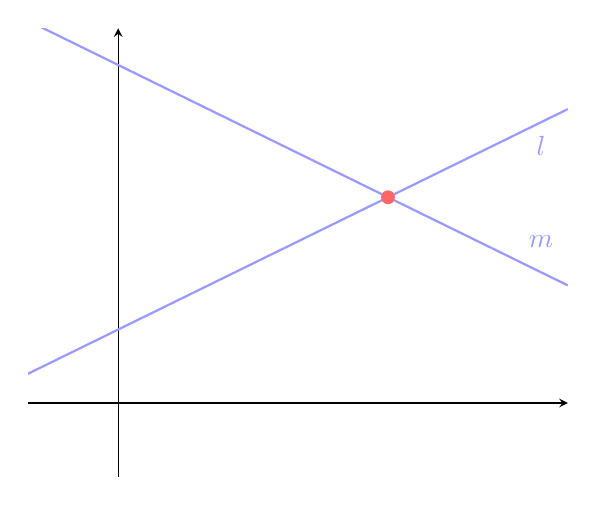
\begin{tikzpicture}
		\begin{axis}[axis lines = middle,
		xmin = -1, 
		ymin = -1,
		ticks = none		
		]
			\addplot[color = blue!40, thick] {0.6*x+1};
			\addplot[color = blue!40, thick] {-0.6*x +4.6};
			\node[color = blue!40] at (axis cs:4.7,3.5) {$l$};
			\node[color = blue!40] at (axis cs: 4.7,2.2) {$m$};
			\node[circle, fill = red!60, inner sep = 0pt, minimum size = 5pt] at (axis cs:
			3,2.8) {};
		\end{axis}
	\end{tikzpicture}
	\caption{Skæring mellem to linjer.}
	\label{fig:linjeligning}
\end{figure}
Lad os betragte et eksempel.
\begin{exa}
	To linjer $l$ og $m$ har ligningerne 
	\begin{align*}
		&l: \ 2(x-1) + 3(y+1) = 0,\\
		&m: \ -4(x+3) + 1(y-2) = 0.
	\end{align*}
	Vi hæver parenteserne i ligningerne:
	\begin{align*}
		&2(x-1)+3(y+1) = 0 \\
		\Leftrightarrow \ &2x-2+3y+3=0\\
		\Leftrightarrow \ &2x+3y+1 = 0
	\end{align*}
	og
	\begin{align*}
		&-4(x+3) + 1(y-2) = 0\\
		\Leftrightarrow \ &-4x-12+y-2 = 0\\
		\Leftrightarrow \ &-4x-14 = -y\\
		\Leftrightarrow \ &y = 4x+14.
	\end{align*}
	Dette indsættes nu på $y$'s plads i første ligning:
	\begin{align*}
		 &2x+3y+1=0\\
		 \Leftrightarrow	\ &2x+3(4x+14) +1 = 0\\
		 \Leftrightarrow	\ &2x + 12x + 42+1 = 0\\
		 \Leftrightarrow \ &14x+43 = 0\\
		 \Leftrightarrow \ &x = -\frac{43}{14}.
	\end{align*}
	Dette indsættes nu i udtrykket for $y$:
	\begin{align*}
		y &= 4x+14 \\
		 &=4\left(\frac{-43}{14}
		\right) + 14\\
		&=\frac{-172}{14} + \frac{196}{14}\\
		&= \frac{24}{14} = \frac{12}{7}
	\end{align*}
	Skæringspunktet mellem linjerne $l$ og $m$ er derfor $\left(\frac{-43}{14},\frac{12}{7}.
	\right)$
\end{exa}

\section*{Skæring givet parametrisering}
\stepcounter{section}
Tilsvarende kan vi også bestemme et skæringspunkt mellem to linjer $l$ og $m$, hvis deres parametrisering er givet. 
\begin{exa}
	Lad $l$ og $m$ være linjer med følgende parametriseringer:
	\begin{align*}
		&l: \ 
		\begin{pmatrix}
			x \\ y
		\end{pmatrix} = 
		\begin{pmatrix}
			4 \\ 4
		\end{pmatrix} + t
		\begin{pmatrix}
			2 \\ -2
		\end{pmatrix},\\
		&m: \ 
		\begin{pmatrix}
			x \\ y 
		\end{pmatrix} = 
		\begin{pmatrix}
			-4 \\ 0
		\end{pmatrix} + t
		\begin{pmatrix}
			5 \\ 1
		\end{pmatrix}.
	\end{align*}
	Vi skal bestemme skæringen mellem disse linjer. Vi sætter dem derfor lig hinanden:
	\begin{align*}
		\begin{pmatrix}
			4 \\ 4
		\end{pmatrix} + t_1
		\begin{pmatrix}
			2 \\ -2
		\end{pmatrix} =
		\begin{pmatrix}
			-4 \\ 0
		\end{pmatrix} + t_2
		\begin{pmatrix}
			5 \\ -1
		\end{pmatrix}.
	\end{align*}
	Dette giver os to lineære ligninger med to ubekendte, som vi enten kan løse med 
	substitution eller ved lige store koefficienters metode. Vi bruger substitutionsmetoden. 
	Ligningerne lyder:
	\begin{align*}
		4 + 2t_1 = -4+5t_2
	\end{align*} og
	\begin{align*}
		4-2t_1 = t_2.
	\end{align*}
	Anden ligning indsættes i første ligning:
	\begin{align*}
		&4 + 2t_1 = -4+5t_2\\
		\Leftrightarrow \ &4 + 2t_1 = -4+5(4-2t_1)\\
		\Leftrightarrow \ &4+2t_1 = -4+20-10t_1\\
		\Leftrightarrow \ &8+2t_1 = 20-10t_1\\
		\Leftrightarrow \ &12t_1 = 12\\
		\Leftrightarrow \ &t_1 = 12.
	\end{align*}
	Dette indsættes i første parameterfremstilling:
	\begin{align*}
		\begin{pmatrix}
			x \\ y
		\end{pmatrix} = 
		\begin{pmatrix}
			4 \\ 4 
		\end{pmatrix} 
		+ 1
		\begin{pmatrix}
			2 \\ -2
		\end{pmatrix} = 
		\begin{pmatrix}
			6 \\ 2
		\end{pmatrix}.
	\end{align*}
	Derfor skærer linjerne $l$ og $m$ hinanden i punktet $(6,2)$. 
\end{exa}

\section*{Opgave 1}
\begin{enumerate}[label=\roman*)]
	\item To linjer $l$ og $m$ har ligningerne
	\begin{align*}
		&l: \ 2(x-2) + 2(y-6) = 0,\\
		&m: \ -1(x-11) + 5(y-3) = 0.
	\end{align*}
	Bestem skæringspunktet mellem $l$ og $m$. 
	\item To linjer $l$ og $m$ har ligningerne 
	\begin{align*}
		&l: \ 2x + 4(y-1) = 0,\\
		&m: \ 2(x-5) -(y-1) = 0.
	\end{align*}
	Bestem skæringspunktet mellem $l$ og $m$.
\end{enumerate}

\section*{Opgave 2}
\begin{enumerate}[label=\roman*)]

\item Bestem skæringen mellem linjerne $l$ og $m$, der har følgende parametriseringer henholdsvist:
\begin{align*}
\begin{pmatrix}
x \\ y
\end{pmatrix}
= 
\begin{pmatrix}
1 \\ -1
\end{pmatrix}
+
t
\begin{pmatrix}
2 \\ 1
\end{pmatrix}
\end{align*}
og 
\begin{align*}
\begin{pmatrix}
x \\ y
\end{pmatrix}
= 
\begin{pmatrix}
-3 \\ 3
\end{pmatrix}
+
t
\begin{pmatrix}
-2 \\ 1
\end{pmatrix}
\end{align*}

\item Bestem skæringen mellem linjerne $l$ og $m$, der har følgende parametriseringer henholdsvist:
\begin{align*}
\begin{pmatrix}
x \\ y
\end{pmatrix}
= 
\begin{pmatrix}
5 \\ 2
\end{pmatrix}
+
t
\begin{pmatrix}
3 \\ 4
\end{pmatrix}
\end{align*}
og 
\begin{align*}
\begin{pmatrix}
x \\ y
\end{pmatrix}
= 
\begin{pmatrix}
-1 \\ 6
\end{pmatrix}
+
t
\begin{pmatrix}
-3 \\ 6
\end{pmatrix}
\end{align*}

\end{enumerate}

\section*{Opgave 3}
\begin{enumerate}[label=\roman*)]
	\item En linje $l$ går gennem punkterne $(1,1)$ og $(2,3)$. Bestem en parametrisering for 
	$l$. 
	\item En linje $m$ går gennem punkterne $(-2,-4)$ og $(3,5)$. Bestem en ligning for $m$. 
\end{enumerate}

\section*{Opgave 4}
\begin{enumerate}[label=\roman*)]
	\item En linje $l$ har parameterfremstillingen 
	\begin{align*}
		\begin{pmatrix}
			x \\ y
		\end{pmatrix} = 
		\begin{pmatrix}
			1 \\ -2
		\end{pmatrix} + t
		\begin{pmatrix}
			2 \\ 1
		\end{pmatrix}
	\end{align*}
	og en anden linje $m$ har ligningen
	\begin{align*}
		(x-3) + 7(y+2) = 0
	\end{align*}
	Bestem skæringspunktet mellem $l$ og $m$. 
	\item En linje $l$ har parameterfremstillingen 
	\begin{align*}
		\begin{pmatrix}
			x \\ y
		\end{pmatrix} = 
		\begin{pmatrix}
			0 \\ 5
		\end{pmatrix} + t
		\begin{pmatrix}
			5 \\ 3
		\end{pmatrix}
	\end{align*}
	og en anden linje $m$ har ligningen
	\begin{align*}
		-5(x+3) + 2(y-2) = 0
	\end{align*}
	Bestem skæringspunktet mellem $l$ og $m$. 
\end{enumerate}
